\section{Introduction}
\label{sec:introduction}

% state the learning objective 
The objective of this laboratory assignment is to study a circuit containing two independent sources, $V_a$ and $I_d$, one voltage controlled source, $I_b$, one current controlled source, $V_c$, connected to seven resistors. The circuit can be seen in Figure~\ref{fig1}.

Labels were assigned to identify nodes from zero to seven to, then proceed with the mesh and node analysis.

In the node analysis, given arbitrary directions to the current in each branch, for each node it was taken the summation of all converging currents, with positive sign, and diverging ones, with negative sign, so that the sum of the currents in all the branches connected to a specific node is zero. Its relevant to notice that this kind of approach is only possible for the nodes which aren't directly connected to a terminal of a voltage source. In that case its crucial to find other equations to cover all the unknown variables of the system.

In the mesh analysis, its given an arbitrary current to each mesh ($I_1$, $I_2$, $I_3$ $I_4$), represented in Figure~\ref{fig1} with round arrows. 



\begin{figure}[h] \centering
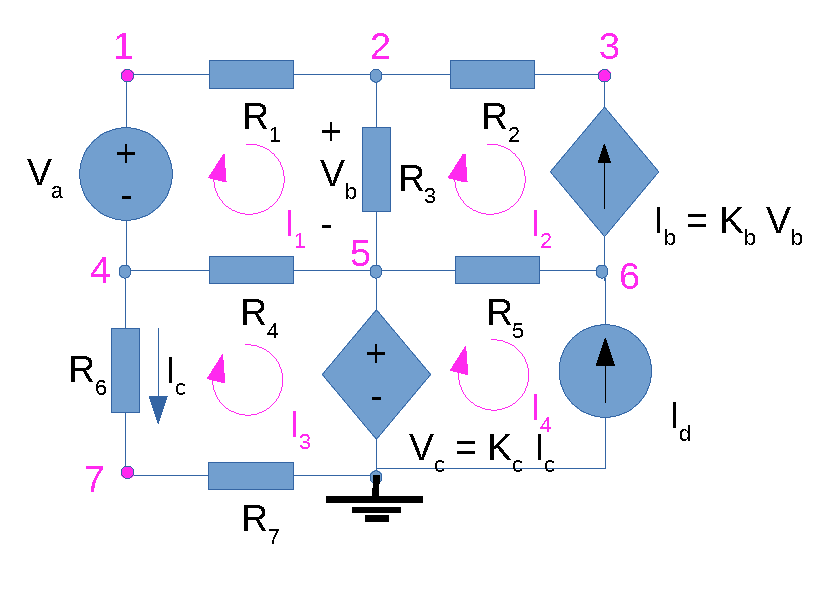
\includegraphics[width=0.4\linewidth]{t1-1.pdf}
\caption{This is circuit that was analysed. The nodes were numbered, as were the currents in each mesh.}
\label{fig1}
\end{figure}

In Section~\ref{sec:analysis}, a theoretical analysis of the circuit is
presented. In Section~\ref{sec:simulation}, the circuit is analysed by
simulation, and the results are compared to the theoretical results obtained in
Section~\ref{sec:analysis}. The conclusions of this study are outlined in
Section~\ref{sec:conclusion}.
